\documentclass{article}

\usepackage[left=2cm,right=2cm,top=2cm,bottom=2cm]{geometry} 

\usepackage[utf8]{inputenc}   % otra alternativa para los caracteres acentuados y la "ñ"
\usepackage[           spanish % para poder usar el español
                      ,es-tabla % para los captions de las tablas
                       ]{babel}   
\decimalpoint %para usar el punto decimal en vez de coma para los números con decimales

%\usepackage{beton}
%\usepackage[T1]{fontenc}

\usepackage{parskip}
\usepackage{xcolor}

\usepackage{caption}

\usepackage{enumerate} % paquete para poder personalizar fácilmente la apariencia de las listas enumerativas

\usepackage{graphicx} % figuras
\usepackage{subfigure} % subfiguras

\usepackage{amsfonts}
\usepackage{amsmath}

\usepackage{listings}
\lstset
{ %Formatting for code in appendix
    language=python,
    basicstyle=\footnotesize,
    stepnumber=1,
    showstringspaces=false,
    tabsize=1,
    breaklines=true,
    breakatwhitespace=false,
}

\definecolor{gris}{RGB}{220,220,220}
	
\usepackage{float} % para controlar la situación de los entornos flotantes

\restylefloat{figure}
\restylefloat{table} 
\setlength{\parindent}{0mm}


\usepackage[bookmarks=true,
            bookmarksnumbered=false, % true means bookmarks in 
                                     % left window are numbered
            bookmarksopen=false,     % true means only level 1
                                     % are displayed.
            colorlinks=true,
            allcolors=blue,
            urlcolor=blue]{hyperref}
\definecolor{webblue}{rgb}{0, 0, 0.5}  % less intense blue

\usepackage[ruled,vlined]{algorithm2e}
\SetKwInOut{Parameter}{parameter}


\title{\Huge Metaheurísticas: Práctica 1 \\ Búsqueda Local y Algoritmos Greedy para el Problema de la Máxima Diversidad \vspace{10mm}}

\author{\huge David Cabezas Berrido \vspace{10mm} \\
	\huge 20079906D \vspace{10mm} \\  
  \huge Grupo 2: Viernes \vspace{10mm} \\ 
  \huge dxabezas@correo.ugr.es \vspace{10mm}}

\begin{document}
\maketitle
\newpage
\tableofcontents
\newpage

\section{Descripción y formulación del problema}

Nos enfrentamos al \textbf{Problema de la Máxima Diversidad} (\textbf{Maximum Diversity Problem, MDP}). El problema consiste en seleccionar
un subconjunto $m$ elementos de un conjunto de $n>m$ elementos de forma que se \textbf{maximice} la \emph{diversidad} entre los
 elementos escogidos.
 
 Disponemos de una matriz $D=(d_{ij})$ de dimensión $n\times n$ que contiene las distancias entre los elementos, la entrada $(i,j)$ contiene el
 valor $d_{ij}$, que corresponde a la distancia entre el elemento $i$-ésimo y el $j$-ésimo. Obviamente, la matriz $D$ es simétrica y con
 diagonal nula.
 
 Existen distintas formas de medir la diversidad, que originan distintas variantes del problema. En nuestro caso, la diversidad será la suma
 de las distancias entre cada par de elementos seleccionados.

De manera formal, se puede formular el problema de la siguiente forma:

\begin{description}
	\item Maximizar 
	\begin{equation} \label{eq:objetivo}
		f(x)=\sum_{i=1}^{n-1}\sum_{j=i+1}^n d_{ij} x_i x_j
	\end{equation}
	\item sujeto a 
	\begin{align*}
		\sum_{i=1}^n x_i &= m \\
		x_i&= \{0,1\}, \quad\forall i=1,\ldots, n.
	\end{align*}
\end{description}

Una solución al problema es un vector binario $x$ que indica qué elementos son seleccionados, seleccionamos el elemento $i$-ésimo si $x_i=1$.

Sin embargo, esta formulación es poco eficiente y para la mayoría de algoritmos proporcionaremos otra equivalente pero más eficiente.

El problema es \textbf{NP-completo} y el tamaño del espacio de soluciones es $\dbinom{n}{m}$, de modo que es conveniente recurrir al uso de metaheurísticas
para atacarlo.

\pagebreak

\section{Aplicación de los algoritmos}

Los algoritmos para resolver este problema tendrán como entradas la matriz $D$ ($n\times n$) y el valor $m$. La salida será un contenedor
(vector, conjunto, \ldots) con los índices de los elementos seleccionados, y no un vector binario como el que utilizamos para la formulación. En nuestro caso utilizaremos conjuntos para representar soluciones.

Para representar las soluciones, usaremos conjuntos de enteros con los elementos seleccionados. La evaluación de la calidad de una solución se hará
sumando la contribución de cada uno de los elementos, y dividiremos la evaluaciónen dos funciones. En lugar de calcular la función evaluación como en
\eqref{eq:objetivo}, lo haremos así:
\begin{equation} \label{eq:objetivo-fact}
f(x)=\frac{1}{2}\sum_{i=1}^{m}\sum_{j=1}^m d(i,j)=\frac{1}{2}\sum_{i=1}^{m}\operatorname{contrib}(i)
\end{equation}
La diferencia es que contamos la distancia entre cada dos elementos $i,j$ dos veces, distancia del elemento $i$-ésimo al $j$-ésimo y del $j$-ésimo al
$i$-ésimo. Esto es obviamente más lento que con $j>i$ en la sumatoria, pero nos permite factorizar la evaluación de la solución como suma de las
 contribuciones de los elementos, lo cuál será útil para reaprovechar cálculos al evaluar soluciones para la Búsqueda Local.
 Además, representar la solución como un vector de $m$ índices y no un vector binario de longitud $n$ presenta una clara ventaja: las sumatorias van hasta
 $m$ en lugar de $n$. No tenemos que computar distancias para luego multiplicarlas por cero como sugería la formulación en \eqref{eq:objetivo}.

Presentamos el pseudocódigo de la función para calcular la contribución de un elemento $x_i$.
\begin{algorithm}
	\DontPrintSemicolon % Some LaTeX compilers require you to use \dontprintsemicolon instead
	\KwIn{Un conjunto de índices $S$.}
	\KwIn{La matriz de distancias $D$.}
	\KwIn{Un entero $e$ correspondiente al índice del elemento.}
	\KwOut{La contribución del elemento $e$, como se describe en \eqref{eq:objetivo-fact}.}
	$contrib \gets 0$\;
	\For{$s$ \textbf{in} $S$} {
		$contrib \gets contrib + D[e,s]$ \tcp*{Sumo las distancias del elemento $e$ a cada elemento de $S$}
	}
	\Return{$contrib$}\;
	\caption{{\sc contrib} calcula la contribución de un elemento en una solución.}
	\label{alg:contrib}
\end{algorithm}

Nótese que el elemento $e$ no tiene que pertenecer al conjunto $S$. Esto obviamente no ocurrirá cuando se vaya a evaluar una solución
al completo invocando esta función con la que describiremos a continuación. Pero, de esta forma, permite conocer cómo influirá en la evaluación el añadir
 un nuevo elemento sin necesidad de añadirlo realmente. 
 
 Ahora presentamos el pseudocódigo de la función para evaluar una solución completa.
 \begin{algorithm}
 	\DontPrintSemicolon % Some LaTeX compilers require you to use \dontprintsemicolon instead
 	\KwIn{Un conjunto de índices $S$.}
 	\KwIn{La matriz de distancias $D$.}
 	\KwOut{El valor de la función objetivo sobre la solución compuesta por $S$, como se describe en \eqref{eq:objetivo-fact}.}
 	$fitness \gets 0$\;
 	\For{$e$ \textbf{in} $S$} {
 		$fitness \gets fitness + \operatorname{contrib}(S,D,e)$ \tcp*{Sumo la contribución de cada elemento de la solución}
 	}
 	\Return{$fitness/2$} \tcp*{Hemos contado cada distancia dos veces} 
 	\caption{{\sc fitness} calcula la evaluación de una solución.}
 	\label{alg:eval}
 \end{algorithm}

Podemos definir la distancia de un elemento $e$ a un conjunto $S$ como:

\begin{equation} \label{eq:distance-elem-set}
	d(e,S)=\sum_{s\in S} d(e,s)
\end{equation}

Esta expresión nos será de utilidad para la implementación de los algoritmos.

Gracias a la existencia del Algoritmo \ref{alg:contrib}, podemos obtener esta expresión como $\operatorname{contrib}(S,D,e)$.

En esta práctica, compararemos los algoritmos Greedy y Búsqueda Local con Primer Mejor. Como trabajo volutario, incluimos también
 la comparación
entre los criterios de búsqueda local \emph{mejor} y \emph{primer mejor}.

\pagebreak

\section{Descripción de los algoritmos}

\subsection{Búsqueda local}

Procedemos con la descripción del algoritmo de Búsqueda Local que se nos ha presentado en el seminario. 
Este algoritmo utiliza la técnica del Primer Mejor, en la que se van generando soluciones en el entorno de la actual y se
salta a la primera con mejor evaluación. Para la implementación del algoritmo, necesitamos distintos elementos.

El primer elemento, es una función para generar una solución aleatoria de partida. Simplemente se eligen $m$ elementos 
diferentes del conjunto. Por comodidad, también calculamos el complementario.

\begin{algorithm}[H]
	\DontPrintSemicolon % Some LaTeX compilers require you to use \dontprintsemicolon instead
	\KwIn{El entero $m$.}
	\KwIn{El entero $n$.}
	\KwOut{Una solución válida del MDP obtenida aleatoriamente.}
	\KwOut{El complementario de la solución obtenida.}
	$E \gets \{0,\ldots, n-1\}$ \tcp*{Conjunto con los elementos no seleccionados}
	$S \gets \emptyset$ \tcp*{La solución empieza vacía}
	\While{$|S|<m$}{
		$e \gets$ elemento aleatorio de $E$\;
		$E \gets E\backslash \{e\}$\;
		$S \gets S\cup \{e\}$\;
	}
	\Return{$S$}\;
	\Return{$E$} \tcp*{El complementario}
	\caption{{\sc RandomSol} proporciona una solución válida aleatoria}
	\label{alg:randomsol}
\end{algorithm}

Lo siguiente que necesitamos es un método para generar las soluciones del entorno. Estas soluciones se consiguen sustituyendo
el menor contribuyente de la solución actual por otro candidato. Presentamos el código para obtener el menor contribuyente.

 \begin{algorithm}[H]
	\DontPrintSemicolon % Some LaTeX compilers require you to use \dontprintsemicolon instead
	\KwIn{Un conjunto de elementos $S$.}
	\KwIn{La matriz de distancias $D$.}
	\KwOut{El elemento de $S$ que minimiza $\operatorname{contrib}(S,S,e)$ con $e\in S$.}
	\KwOut{Su contribución, para la factorización de la función objetivo.}
	$lowest \gets \text{primer elemento de } S$\;
	$min\_contrib \gets \operatorname{contrib}(S,D,lowest)$\;
	\For{$s$ \textbf{in} $S$} {
		$contrib \gets \operatorname{contrib}(S,D,s)$\;
		\If{$contrib < min\_contrib$} { 
			$min\_contrib \gets contrib$\;
			$lowest \gets s$ \tcp*{Si encuentro un candidato con menor contribución, actualizo}
		}
	}
	\Return{$lowest$}\;
	\Return{$min\_contrib$}\;
	\caption{{\sc lowestContrib} obtiene el elemento de $S$ que menos contribuye en la valoración.}
	\label{alg:lowest-contributor}
\end{algorithm}

En el caso de que $S$ se represente como un conjunto, no sabemos cuál será el primer elemento (depende de la implementación del iterador). Pero
esto no es relevante, ya que vale cualquier elemento de $S$.

Finalmente, proporcionamos el algoritmo de Búsqueda Local para actualizar la solución por otra del entorno iterativamente
hasta encontrar un máximo local (una solución mejor que todas las de su entorno) ollegar a un límite de evaluaciones de la función
 objetivo: $LIMIT=100000$. Las soluciones del entorno se generan aleatoriamente.

\begin{algorithm}[H]
	\DontPrintSemicolon % Some LaTeX compilers require you to use \dontprintsemicolon instead
	\KwIn{El entero $m$.}
	\KwIn{La matriz de distancias $D$, $n\times n$.}
	\KwOut{Una solución válida del MDP por el algoritmo de BS que hemos descrito, junto con su evaluación.}
	$S \gets \operatorname{randomSol}(m,n)$ \tcp*{Comenzamos con una solución aleatoria}
	$E \gets \{0,\ldots,n-1\}\backslash S$ \tcp*{$\operatorname{randomSol}$ también devuelve el complementario}
	$fitness \gets \operatorname{fitness}(S)$ \tcp*{Diversidad de la solución}
	$E \gets \operatorname{vector}(E)$ \tcp*{No importa el orden, pero debe poder barajarse}
	$carryon \gets true$\;
	$LIMIT \gets 100000$ \tcp*{Límite de llamadas a la función de evaluación}
	$CALLS \gets 0$\;
	\While{carryon}{
		$lowest = \operatorname{lowestContributor}(S,D)$\;
		$min\_contrib \gets \operatorname{contrib}(S,D,lowest)$ \tcp*{Se calcula dentro de $\operatorname{lowestContributor}$}
		$S \gets S\backslash\{lowest\}$\;
		$E \gets \operatorname{shuffle}(E)$\;	
		\For{$e$ \textbf{in} $E$} {
			$contrib \gets \operatorname{contrib}(S,D,e)$\;
			$CALLS \gets CALLS +1$ \tcp*{He evaludado una posible solución}
			\If{$contrib > min\_contrib$} { 
				$fitness \gets fitness + contrib - min\_contrib$ \tcp*{Diversidad de la nueva solución}
				$carryon \gets true$ \tcp*{Toca saltar, lo que completa la iteración}
				$S\gets S\cup\{e\}$ \tcp*{Saltamos a la nueva solución}
				$E \gets E\backslash\{e\}$\;
				$E \gets E\cup\{lowest\}$\;
			}
			\If{$carryon==true$ or $CALLS\geq LIMIT$} { 
				\textbf{break}  \tcp*{Se cumple alguna de las condiciones de parada}
			}
		}
	}
	\If{$|S|<m$} { 
		$S\gets S\cup\{lowest\}$ \tcp*{Si salimos porque no encontramos una mejor, recuperamos la solución}
	}
	\Return{$S$}\;
	\Return{$fitness$}\;
	\caption{{\sc LocalSearch}}
	\label{alg:local-search}
\end{algorithm}

Cabe destacar que a diferencia del algoritmo Greedy (Algoritmo \ref{alg:greedy}) en el que se evalúa la solución al final,
en este algoritmo se calcula factorizando. Esto acelera mucho los cálculos, ya que hay que evaluar muchas soluciones diferentes.

\pagebreak

\section{Algoritmo de comparación: Greedy}

Para comparar la eficacia de cada algoritmos, lo compararemos con el algoritmo \textbf{Greedy} descrito en el seminario.

El algoritmo consiste en empezar por el elemento más lejano al resto e ir añadiendo el elemento que más contribuya hasta completar una solución
válida.

Como elemento más lejano al resto se toma el elemento cuya suma de las distancias al resto sea la mayor. Y en cada iteración se introduce el elemento
cuya suma de las distancias a los seleccionados sea mayor. Es decir, utilizamos la definición de \eqref{eq:distance-elem-set}.

Para calcular ambos valores, usamos la siguiente función, que permite obtener el de entre
un conjunto de candidatos más lejano (en el sentido que acabamos de comentar) a los elementos de un conjunto dado.
El código para calcularlo es similar al del algoritmo \ref{alg:lowest-contributor}.

 \begin{algorithm}[H]
	\DontPrintSemicolon % Some LaTeX compilers require you to use \dontprintsemicolon instead
	\KwIn{Un conjunto de candidatos $C$.}
	\KwIn{Un conjunto de elementos $S$.}
	\KwIn{La matriz de distancias $D$.}
	\KwOut{El candidato más lejano en el sentido de \eqref{eq:distance-elem-set}.}
	$farthest \gets \text{primer elemento de } C$\;
	$max\_contrib \gets \operatorname{contrib}(S,D,farthest)$\;
	\For{$e$ \textbf{in} $C$} {
		$contrib \gets \operatorname{contrib}(S,D,e)$\;
		\If{$contrib > max\_contrib$} { 
			$max\_contrib \gets contrib$\;
			$farthest \gets e$ \tcp*{Si encuentro un candidato con mayor contribución, actualizo}
		}
	}
	\Return{$farthest$}\;
	\caption{{\sc farthest} obtiene el candidato más lejano a los elementos de $S$.}
	\label{alg:farthest-candidate-set}
\end{algorithm}

En el caso de que $C$ se represente como un conjunto, no sabemos cuál será el primer elemento (depende de la implementación del iterador). Pero
esto no es relevante, ya que vale cualquier elemento de $C$.

Ya estamos en condiciones de proporcionar una descripción del algoritmo Greedy.

 \begin{algorithm}[H]
	\DontPrintSemicolon % Some LaTeX compilers require you to use \dontprintsemicolon instead
	\KwIn{La matriz de distancias $D$.}
	\KwIn{El entero $m$.}
	\KwOut{Una solución válida del MDP obtenida como hemos descrito anteriormente, y su diversidad.}
	$C \gets \{0,\ldots, n-1\}$ \tcp*{En principio los $n$ elementos son candidatos}
	$S \gets \emptyset$ \tcp*{La solución empieza vacía}
	$farthest \gets \operatorname{farthest}(C,C,D)$ \tcp*{Elemento más lejano al resto}
	$C \gets C\backslash \{farthest\}$\;
	$S \gets S\cup \{farthest\}$\;
	\While{$|S|<m$}{
		$farthest \gets \operatorname{farthest}(C,S,D)$ \tcp*{Elemento más lejano a los seleccionados}
		$C \gets C\backslash \{farthest\}$\;
		$S \gets S\cup \{farthest\}$\;
	}
	\Return{$S$}\;
	\Return{$\operatorname{fitness}(S)$}\;
	\caption{{\sc Greedy}}
	\label{alg:greedy}
\end{algorithm}

\pagebreak

\section{Desarrollo de la práctica}

La implementación de los algoritmos y la experimentación con los mismos se ha llevado acabo de C++, utilizando la librería STL. 
Para representar la soluciones hemos hecho uso del tipo \texttt{unordered\_set}, ya que se realizan pocas operaciones de consulta y
muchas de inserción y borrado.

Para medir los tiempos de ejecución se utiliza la función \texttt{clock} de la librería \texttt{time.h}.

A lo largo de la práctica se utilizan acciones aleatorias. Utilizamos la librería \texttt{stdlib.h} para la generación de
números pseudoaleatorios con \texttt{rand} y fijamos la semilla con \texttt{srand}. También se baraja el vector de candidatos
en la búsqueda local con la función \texttt{random\_shuffle} de la librería \texttt{algorithm}.

Se almacena la matriz de distancias completa (no sólo un triángulo) por comodidad de los cálculos.

\subsection{Manual de usuario}

A continuación detallamos instrucciones para lanzar los ejecutables.

Tenemos los siguientes ejecutables:

\begin{itemize}
	\item \textbf{Greedy:} Implementación del algoritmo Greedy.
	\item \textbf{LocalSearch:} Implementación del algoritmo de Búsqueda Local (Primer Mejor).
	\item \textbf{LocalSearch2:} Implementación del algoritmo de Búsqueda Local (Mejor).
\end{itemize}

Todos ellos devuelven la evaluación de la solución obtenida y el tiempo de ejecución por salida estándar.
Leen el fichero por entrada estándar, así que es conveniente redirigirla.

Ejemplo:
\begin{verbatim}
	bin/greedy < datos/MDG-a_1_n500_m50.txt >> salidas/greedy.txt
\end{verbatim}

Los programas correspondientes a la búsqueda local, también devuelven el número de llamadas a la función de evaluación, para
comparar cómo de cerca se quedan del límite.

Tenemos dos ejecutables más: \textbf{LocalSearchEvol} y \textbf{LocalSearch2Evol}, que son versiones equivalentes a
\textbf{LocalSearch} y \textbf{LocalSearch2}, pero con la diferencia de que devuelven una lista con la fitness de la solución
en cada iteración. Los usamos para estudiar la evolución de la solución a lo largo del proceso y obtener gráficas de convergencia.

Además, todos los archivos de búsqueda locall reciben la semilla como parámetro. Ejemplo:
\begin{verbatim}
bin/localSearch 197 < datos/MDG-a_1_n500_m50.txt >> salidas/localSearch.txt
\end{verbatim}

En la carpeta \textbf{software} se incluye el script usado para lanzar todas las ejecuciones, \texttt{run.sh}.

\pagebreak

\section{Experimentación y análisis}

Toda la experimentación se realiza en mi ordenador portátil personal, que tiene las siguientes especificaciones:
\begin{itemize}
	\item OS: Ubuntu 20.04.2 LTS x86\_64.
	\item RAM: 8GB, DDR4.
	\item CPU: Intel Core i7-6700HQ, 2.60Hz.
\end{itemize}

\subsection{Casos de estudio y resultados}

Tratamos varios casos con distintos parámetros $n$ y $m$. En cada caso se utiliza una semilla diferente para Búsqueda Local.
A continuación presentamos una tabla con los casos estudiados. Para cada caso indicamos los valores de $n$ y $m$ y la semilla
que se utiliza para la búsqueda local.

\begin{table}[H]
	\centering
	\begin{tabular}{|cccc|}
		\hline
		Caso & $n$ & $m$ & Seed\\ \hline
		MDG-a\_10\_n500\_m50 & 500 & 50 & 13\\
		MDG-a\_1\_n500\_m50 & 500 & 50 & 19\\
		MDG-a\_2\_n500\_m50 & 500 & 50 & 25\\
		MDG-a\_3\_n500\_m50 & 500 & 50 & 31\\
		MDG-a\_4\_n500\_m50 & 500 & 50 & 37\\
		MDG-a\_5\_n500\_m50 & 500 & 50 & 43\\
		MDG-a\_6\_n500\_m50 & 500 & 50 & 49\\
		MDG-a\_7\_n500\_m50 & 500 & 50 & 55\\
		MDG-a\_8\_n500\_m50 & 500 & 50 & 61\\
		MDG-a\_9\_n500\_m50 & 500 & 50 & 67\\
		MDG-b\_21\_n2000\_m200 & 2000 & 200 & 73\\
		MDG-b\_22\_n2000\_m200 & 2000 & 200 & 79\\
		MDG-b\_23\_n2000\_m200 & 2000 & 200 & 85\\
		MDG-b\_24\_n2000\_m200 & 2000 & 200 & 91\\
		MDG-b\_25\_n2000\_m200 & 2000 & 200 & 97\\
		MDG-b\_26\_n2000\_m200 & 2000 & 200 & 103\\
		MDG-b\_27\_n2000\_m200 & 2000 & 200 & 109\\
		MDG-b\_28\_n2000\_m200 & 2000 & 200 & 115\\
		MDG-b\_29\_n2000\_m200 & 2000 & 200 & 121\\
		MDG-b\_30\_n2000\_m200 & 2000 & 200 & 127\\
		MDG-c\_10\_n3000\_m400 & 3000 & 400 & 133\\
		MDG-c\_13\_n3000\_m500 & 3000 & 500 & 139\\
		MDG-c\_14\_n3000\_m500 & 3000 & 500 & 145\\
		MDG-c\_15\_n3000\_m500 & 3000 & 500 & 151\\
		MDG-c\_19\_n3000\_m600 & 3000 & 600 & 157\\
		MDG-c\_1\_n3000\_m300 & 3000 & 300 & 163\\
		MDG-c\_20\_n3000\_m600 & 3000 & 600 & 169\\
		MDG-c\_2\_n3000\_m300 & 3000 & 300 & 175\\
		MDG-c\_8\_n3000\_m400 & 3000 & 400 & 181\\
		MDG-c\_9\_n3000\_m400 & 3000 & 400 & 187\\
		\hline
	\end{tabular}
\caption{Tabla con los parámetros y semillas de cada caso. Ordenando los nombres de los ficheros por orden alfabético
(el orden en el que los procesa el script), las semillas son números del 13 al 187 saltando de 6 en 6.}
\label{tab:param-seed}
\end{table}

Ahora mostraremos para cada algoritmo una tabla con los estadísticos (Desviación y Tiempo) que han obtenido en cada
caso.

\pagebreak

Comenzamos con el algoritmo \textbf{Greedy}.

\begin{table}[H]
	\centering
	\begin{tabular}{|cccc|}
		\hline
		Caso & Coste obtenido & Desv & Tiempo (s)\\ \hline
		MDG-a\_1\_n500\_m50 & 7610.42 & 2.85 & 0.001375\\
		MDG-a\_2\_n500\_m50 & 7574.39 & 2.54 & 0.001293\\
		MDG-a\_3\_n500\_m50 & 7535.96 & 2.88 & 0.001304\\
		MDG-a\_4\_n500\_m50 & 7551.52 & 2.81 & 0.001281\\
		MDG-a\_5\_n500\_m50 & 7540.14 & 2.77 & 0.001284\\
		MDG-a\_6\_n500\_m50 & 7623.65 & 1.93 & 0.001278\\
		MDG-a\_7\_n500\_m50 & 7594.62 & 2.28 & 0.0014\\
		MDG-a\_8\_n500\_m50 & 7625.94 & 1.61 & 0.001367\\
		MDG-a\_9\_n500\_m50 & 7547.25 & 2.87 & 0.001351\\
		MDG-a\_10\_n500\_m50 & 7642.27 & 1.77 & 0.001893\\
		MDG-b\_21\_n2000\_m200 & 11099332.620328 & 1.77 & 0.319017\\
		MDG-b\_22\_n2000\_m200 & 11149879.733826 & 1.21 & 0.313017\\
		MDG-b\_23\_n2000\_m200 & 11119613.974858 & 1.6 & 0.303374\\
		MDG-b\_24\_n2000\_m200 & 11106996.970212 & 1.63 & 0.311278\\
		MDG-b\_25\_n2000\_m200 & 11114220.292214 & 1.61 & 0.306411\\
		MDG-b\_26\_n2000\_m200 & 11132801.799043 & 1.41 & 0.306542\\
		MDG-b\_27\_n2000\_m200 & 11130608.965587 & 1.55 & 0.310595\\
		MDG-b\_28\_n2000\_m200 & 11110673.520354 & 1.5 & 0.318429\\
		MDG-b\_29\_n2000\_m200 & 11156328.082493 & 1.25 & 0.306362\\
		MDG-b\_30\_n2000\_m200 & 11109767.818822 & 1.65 & 0.296905\\
		MDG-c\_1\_n3000\_m300 & 24617010 & 1.07 & 1.501668\\
		MDG-c\_2\_n3000\_m300 & 24547293 & 1.44 & 1.464132\\
		MDG-c\_8\_n3000\_m400 & 43056071 & 0.88 & 2.546235\\
		MDG-c\_9\_n3000\_m400 & 42958639 & 1.1 & 2.569214\\
		MDG-c\_10\_n3000\_m400 & 42959794 & 1.19 & 2.566065\\
		MDG-c\_13\_n3000\_m500 & 66493045 & 0.78 & 3.67213\\
		MDG-c\_14\_n3000\_m500 & 66449858 & 0.79 & 3.767131\\
		MDG-c\_15\_n3000\_m500 & 66468837 & 0.78 & 3.78725\\
		MDG-c\_19\_n3000\_m600 & 94929882 & 0.74 & 5.183856\\
		MDG-c\_20\_n3000\_m600 & 94979205 & 0.69 & 5.582157\\
		\hline
	\end{tabular}
	\caption{Evaluación de las soluciones y estadísticos \emph{Desv} y \emph{Tiempo} obtenidos por el algoritmo Greedy
		en cada caso de estudio.}
	\label{tab:greedy}
\end{table}

Media de los estadísticos:
\begin{table}[H]
	\centering
	\begin{tabular}{|cc|}
		\hline
		Desv & Tiempo (s)\\ \hline
		1.63 & 1.19 \\
		\hline
	\end{tabular}
\end{table}

\pagebreak

Ahora pasamos al algoritmo de \textbf{Búsqueda Local}.

\begin{table}[H]
	\centering
	\begin{tabular}{|cccc|}
		\hline
		Caso & Coste obtenido & Desv & Tiempo (s)\\ \hline
		MDG-a\_1\_n500\_m50 & 7623.23 & 2.69 & 0.001809\\
		MDG-a\_2\_n500\_m50 & 7590.18 & 2.34 & 0.001391\\
		MDG-a\_3\_n500\_m50 & 7544.94 & 2.76 & 0.001204\\
		MDG-a\_4\_n500\_m50 & 7576.44 & 2.49 & 0.0012\\
		MDG-a\_5\_n500\_m50 & 7484.27 & 3.49 & 0.001308\\
		MDG-a\_6\_n500\_m50 & 7570.96 & 2.61 & 0.001297\\
		MDG-a\_7\_n500\_m50 & 7654.98 & 1.5 & 0.001608\\
		MDG-a\_8\_n500\_m50 & 7623.78 & 1.64 & 0.002379\\
		MDG-a\_9\_n500\_m50 & 7612.74 & 2.02 & 0.001494\\
		MDG-a\_10\_n500\_m50 & 7619.52 & 2.07 & 0.001959\\
		MDG-b\_21\_n2000\_m200 & 11181874.0007 & 1.04 & 0.099777\\
		MDG-b\_22\_n2000\_m200 & 11167876.184 & 1.05 & 0.092492\\
		MDG-b\_23\_n2000\_m200 & 11176568.0611 & 1.09 & 0.107634\\
		MDG-b\_24\_n2000\_m200 & 11188223.318 & 0.91 & 0.107425\\
		MDG-b\_25\_n2000\_m200 & 11181859.8196 & 1.01 & 0.090053\\
		MDG-b\_26\_n2000\_m200 & 11193478.832 & 0.88 & 0.122694\\
		MDG-b\_27\_n2000\_m200 & 11211629.6839 & 0.83 & 0.112468\\
		MDG-b\_28\_n2000\_m200 & 11151089.4629 & 1.14 & 0.079449\\
		MDG-b\_29\_n2000\_m200 & 11183039.6644 & 1.01 & 0.09833\\
		MDG-b\_30\_n2000\_m200 & 11159590.8213 & 1.21 & 0.090033\\
		MDG-c\_1\_n3000\_m300 & 24729057 & 0.62 & 0.601221\\
		MDG-c\_2\_n3000\_m300 & 24738675 & 0.67 & 0.584432\\
		MDG-c\_8\_n3000\_m400 & 43200330 & 0.55 & 1.264437\\
		MDG-c\_9\_n3000\_m400 & 43157977 & 0.64 & 1.241837\\
		MDG-c\_10\_n3000\_m400 & 43188306 & 0.66 & 1.195051\\
		MDG-c\_13\_n3000\_m500 & 66636142 & 0.56 & 2.304507\\
		MDG-c\_14\_n3000\_m500 & 66727635 & 0.38 & 2.430114\\
		MDG-c\_15\_n3000\_m500 & 66808383 & 0.28 & 2.78715\\
		MDG-c\_19\_n3000\_m600 & 95244690 & 0.41 & 3.572005\\
		MDG-c\_20\_n3000\_m600 & 95324379 & 0.33 & 3.598978\\
		\hline
	\end{tabular}
	\caption{Evaluación de las soluciones y estadísticos \emph{Desv} y \emph{Tiempo} obtenidos por el algoritmo de Búsqueda Local
		con Primer Mejor en cada caso de estudio.}
	\label{tab:bs-primer-mejor}
\end{table}

Media de los estadísticos:
\begin{table}[H]
	\centering
	\begin{tabular}{|cc|}
		\hline
		Desv & Tiempo (s)\\ \hline
		1.3 & 0.69 \\
		\hline
	\end{tabular}
\end{table}

Comparamos los estadísticos medios obtenidos por ambos algoritmos.

\begin{table}[H]
	\centering
	\begin{tabular}{|ccc|}
		\hline
		Algoritmo & Desv & Tiempo (s)\\ \hline
		Greedy & 1.63 & 1.19 \\
		BL & 1.3 & 0.69 \\
		\hline
	\end{tabular}
	\caption{Comparativa de los estadísticos medios obtenidos por el algoritmo Greedy y por el de Búsqueda Local.}
	\label{tab:comparativa}
\end{table}

\pagebreak

\subsection{Análisis de resultados}

A la vista de la Tabla \ref{tab:comparativa}, intuimos que ambos algoritmos son adecuados para el problema.
El algoritmo Greedy, en media, alcanza el 98.37\% de la diversidad de la mejor solución posible. Mientras que la Búsqueda Local
 alcanza el 98.7\%.
 
 La BL resulta ser algo más efectiva, debido a que explora el espacio de soluciones con una mayor profundidad que Greedy.
 
 En las Tablas \ref{tab:greedy} y \ref{tab:bs-primer-mejor}, observamos que la desviación es menor en los casos con mayores 
 valores de $n$ y $m$. En general, es algo superior a 2 en los 10 ejemplos del grupo MDG-a, algo inferior a 2 para Greedy y
 cercana a 1 para BL en los 10 ejemplos del grupo MDG-b y algo inferior a 1 (entorno a 0.8 para Greedy y 0.55 para BL) en los 10
  ejemplos del grupo MDG-c. En la gran mayoría de casos, mejor la Búsqueda Local.
  
  Además, observamos que la mejora de la Búsqueda Local respecto a Greedy se acentúa en ejemplos con mayor número de elementos,
  al menos en términos
  relativos. Ya que una mejora del 0.25\% en la desviación cuando los algoritmos rondan desviaciones del 0.65 es bastante
   significativo, más que mejorar en 0.5\% cuando rondan desviaciones de 1.5 ó 2. Parece que cuanto mayor es el espacio de
   búsqueda, la mayor profundidad de exploración de BL cobra más relevancia.
   
  En cuanto al tiempo, nos sorprende la rapidez de la Búsqueda Local, que de media tarda un poco más de la mitad que Greedy.
  
  La mayor parte del tiempo de cómputo en el algoritmo Greedy se invierte en iterar sobre los elementos no seleccionados
   (prácticamente $n$) para encontrar el más lejano a los seleccionados. En cambio, en la Búsqueda Local sólo se itera hasta
   encontrar un candidato mejor que el peor de los seleccionados, aunque se evalúan soluciones completas.
   En el algoritmo Greedy se evalúa la solución completa al final.
   
   Otra fracción muy importante del tiempo de cómputo de Búsqueda Local se invierte también en barajar el vector de candidatos,
   que son $n-m$, para explorar los entornos de las soluciones de forma aleatoria. Hay que barajar por cada actualización de la
   solución.
   
   El motivo por que el la Búsqueda Local sea mucho más rápida es la factorización de la función de evaluación. Aunque técnicamente
   estemos evaluando nuevas soluciones completas, ya conocemos la contribución de todos los candidatos menos el posible nuevo
   seleccionado. Esto hace que el cálculo sea equivalente al de probar un nuevo candidato de Greedy.
   
   De todos modos, podemos considerar que ambos algoritmos son rápidos. Los tiempos de ejecución no han supuesto ningún impedimento
   en el desarrollo de la práctica, han sido prácticamente despreciables.
   
   A continuación incluiremos gráficas de convergencia para analizar la evolución de las soluciones de BL a medida que el algoritmo
   avanza.
   
\pagebreak
   
\subsubsection{Gráficas de convergencia}

Mostramos en gráficas el valor de la función de evaluación sobre la solución en cada actualización de la Búsqueda Local.

\begin{figure}[H]
	\centering
	\subfigure{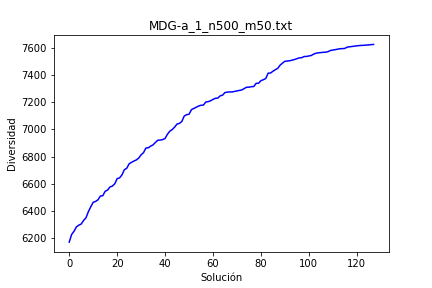
\includegraphics[width=57.5mm]{imgs/LSEvol/LSEMDG-a-1-n500-m50}}
	\subfigure{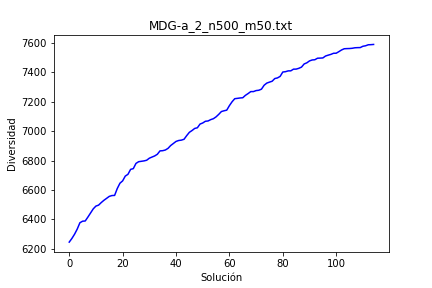
\includegraphics[width=57.5mm]{imgs/LSEvol/LSEMDG-a-2-n500-m50}}
	\subfigure{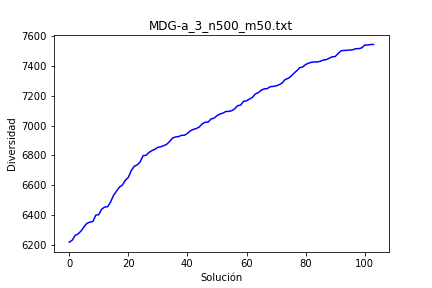
\includegraphics[width=57.5mm]{imgs/LSEvol/LSEMDG-a-3-n500-m50}}
	\subfigure{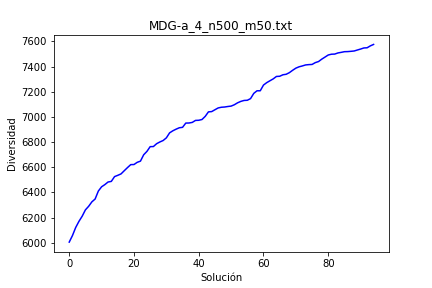
\includegraphics[width=57.5mm]{imgs/LSEvol/LSEMDG-a-4-n500-m50}}
	\subfigure{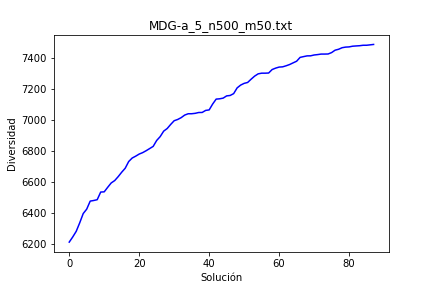
\includegraphics[width=57.5mm]{imgs/LSEvol/LSEMDG-a-5-n500-m50}}
	\subfigure{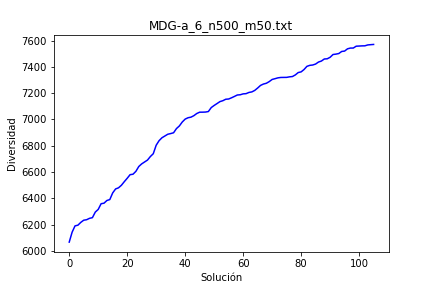
\includegraphics[width=57.5mm]{imgs/LSEvol/LSEMDG-a-6-n500-m50}}
	\subfigure{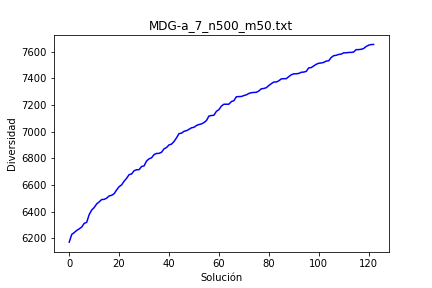
\includegraphics[width=57.5mm]{imgs/LSEvol/LSEMDG-a-7-n500-m50}}
	\subfigure{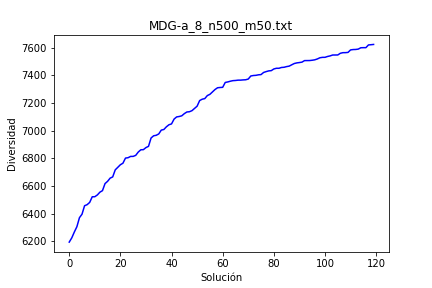
\includegraphics[width=57.5mm]{imgs/LSEvol/LSEMDG-a-8-n500-m50}}
	\subfigure{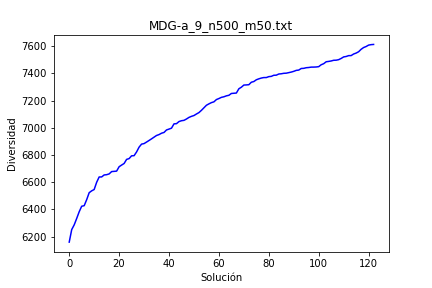
\includegraphics[width=57.5mm]{imgs/LSEvol/LSEMDG-a-9-n500-m50}}
	\subfigure{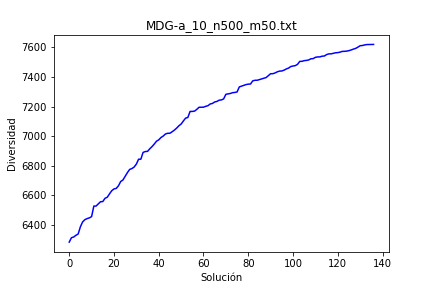
\includegraphics[width=57.5mm]{imgs/LSEvol/LSEMDG-a-10-n500-m50}}
	\caption{Gráficas de convergencia de BL con Primer Mejor en los ejemplos del grupo MDG-a.}
	\label{fig:graph-bl-firstbest-a}
\end{figure}

\begin{figure}[H]
	\centering
	\subfigure{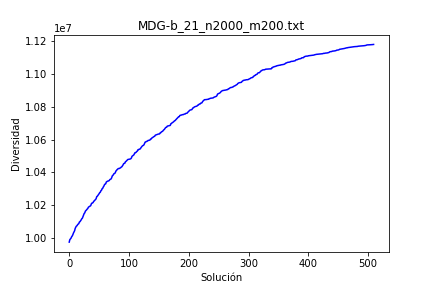
\includegraphics[width=57.5mm]{imgs/LSEvol/LSEMDG-b-21-n2000-m200}}
	\subfigure{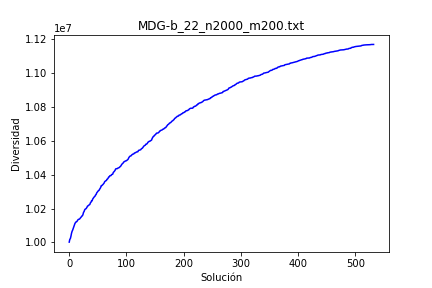
\includegraphics[width=57.5mm]{imgs/LSEvol/LSEMDG-b-22-n2000-m200}}
	\subfigure{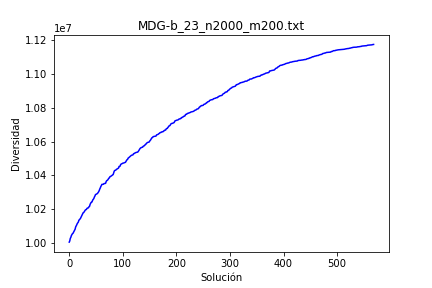
\includegraphics[width=57.5mm]{imgs/LSEvol/LSEMDG-b-23-n2000-m200}}
	\subfigure{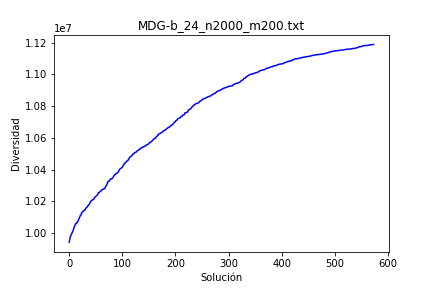
\includegraphics[width=57.5mm]{imgs/LSEvol/LSEMDG-b-24-n2000-m200}}
	\subfigure{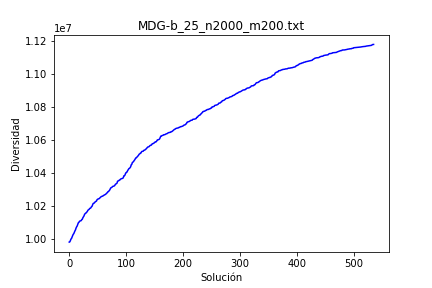
\includegraphics[width=57.5mm]{imgs/LSEvol/LSEMDG-b-25-n2000-m200}}
	\subfigure{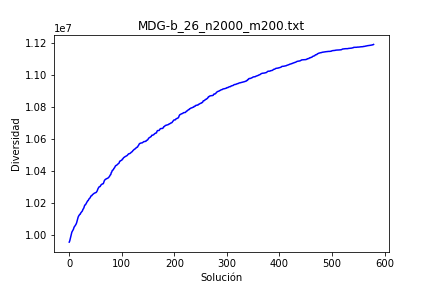
\includegraphics[width=57.5mm]{imgs/LSEvol/LSEMDG-b-26-n2000-m200}}
	\subfigure{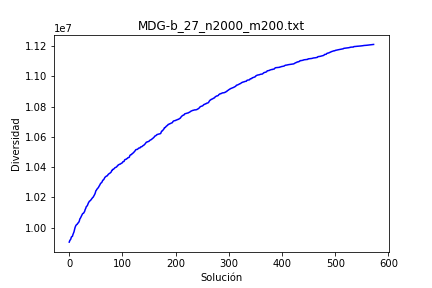
\includegraphics[width=57.5mm]{imgs/LSEvol/LSEMDG-b-27-n2000-m200}}
	\subfigure{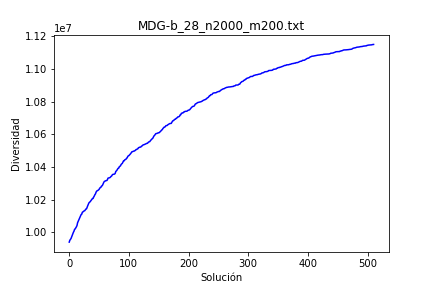
\includegraphics[width=57.5mm]{imgs/LSEvol/LSEMDG-b-28-n2000-m200}}
	\subfigure{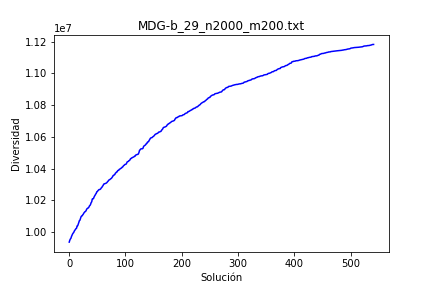
\includegraphics[width=57.5mm]{imgs/LSEvol/LSEMDG-b-29-n2000-m200}}
	\subfigure{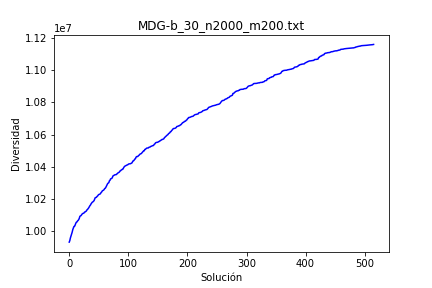
\includegraphics[width=57.5mm]{imgs/LSEvol/LSEMDG-b-30-n2000-m200}}
	\caption{Gráficas de convergencia de BL con Primer Mejor en los ejemplos del grupo MDG-b.}
	\label{fig:graph-bl-firstbest-b}
\end{figure}

\begin{figure}[H]
	\centering
	\subfigure{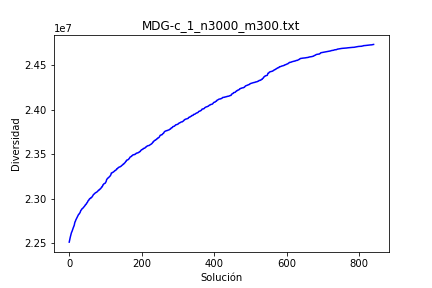
\includegraphics[width=57.5mm]{imgs/LSEvol/LSEMDG-c-1-n3000-m300}}
	\subfigure{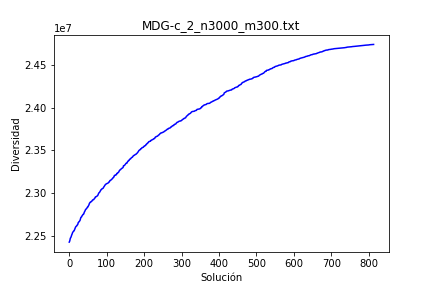
\includegraphics[width=57.5mm]{imgs/LSEvol/LSEMDG-c-2-n3000-m300}}
	\subfigure{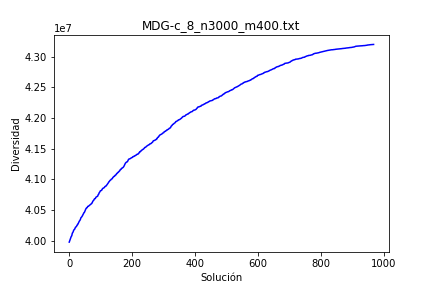
\includegraphics[width=57.5mm]{imgs/LSEvol/LSEMDG-c-8-n3000-m400}}
	\subfigure{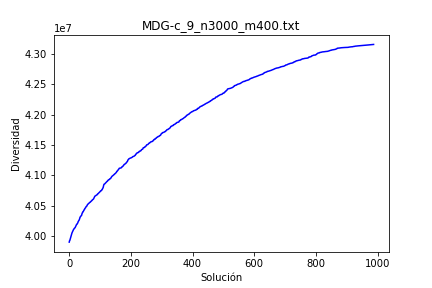
\includegraphics[width=57.5mm]{imgs/LSEvol/LSEMDG-c-9-n3000-m400}}
	\subfigure{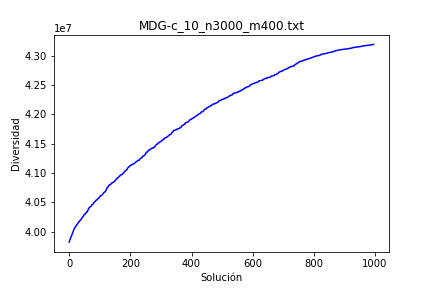
\includegraphics[width=57.5mm]{imgs/LSEvol/LSEMDG-c-10-n3000-m400}}
	\subfigure{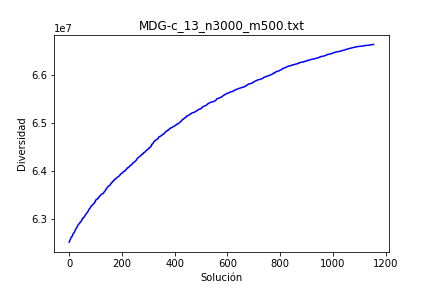
\includegraphics[width=57.5mm]{imgs/LSEvol/LSEMDG-c-13-n3000-m500}}
	\subfigure{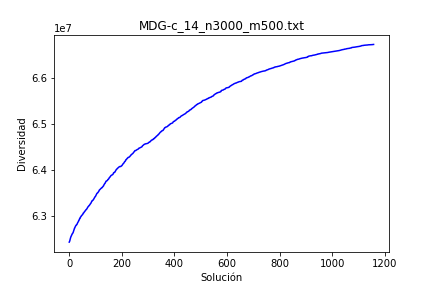
\includegraphics[width=57.5mm]{imgs/LSEvol/LSEMDG-c-14-n3000-m500}}
	\subfigure{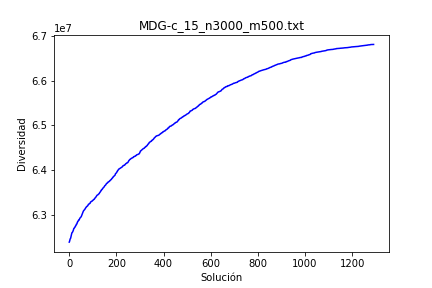
\includegraphics[width=57.5mm]{imgs/LSEvol/LSEMDG-c-15-n3000-m500}}
	\subfigure{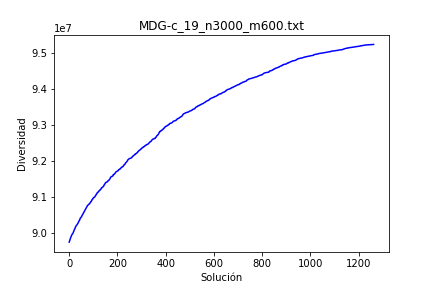
\includegraphics[width=57.5mm]{imgs/LSEvol/LSEMDG-c-19-n3000-m600}}
	\subfigure{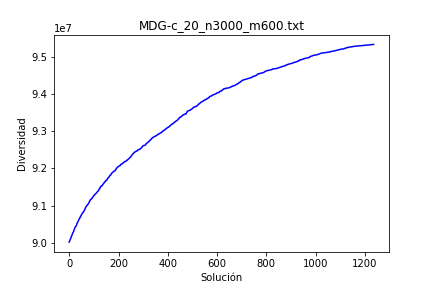
\includegraphics[width=57.5mm]{imgs/LSEvol/LSEMDG-c-20-n3000-m600}}
	\caption{Gráficas de convergencia de BL con Primer Mejor en los ejemplos del grupo MDG-c.}
	\label{fig:graph-bl-firstbest-c}
\end{figure}

En general, observamos que la mejora es mayor en las primeras iteraciones, lo que les da a las gráficas una característica forma
creciente y cóncava.

En el eje de abscisas de cada gráfica podemos apreciar el número de actualizaciones que han tenido lugar durante el desarollo del
 algoritmo.
Es del orden de unas 100 para los ejemplos de MDG-a, 500-600 para los de MDG-b y entre 800 y 1000 para los de MDG-c. Hay que 
tener en cuenta que la estrategia del Primer Mejor da lugar a una gran cantidad de actualizaciones, con pequeña mejoría de
una actualización a la siguiente.

En los ejes de ordenadas se observa la mejora de diversidad que consigue el algoritmo partiendo de la solución aleatoria. Esta mejora ronda el 
20-25\% para los ejemplos del grupo MDG-a, es entorno al 12\% para los ejemplos del grupo MDG-b, y de ligeramente menos del 10\%
para los del grupo MDG-c. Esto le resta importancia al hecho de que los algoritmos hayan conseguido desviaciones más bajas en los
ejemplos grandes, pues una solución aleatoria también presenta menos desviación en los ejemplos grandes que en los pequeños.

\pagebreak

\section{Trabajo voluntario}

\subsection{Comparación Búsqueda Local: Mejor vs Primer Mejor}

En el seminario se nos ha aconsejado la estrategia del Primer Mejor para la Búsqueda Local, que consiste en actualizar una
solución cuando se encuentra una mejor en su entorno. La comparamos con la estrategia del Mejor, que explora todo el entorno
de cada solución y salta a la mejor solución del entorno.

A priori, tenemos una ventaja y dos inconvenientes. Por una parte, saltar a la mejor solución posible del entorno hace que el
valor de la función de evaluación crezca más rápido, lo que conlleva tener que realizar menos actualizaciones y menos barajamientos
del vector de no seleccionados.

Por otra parte, exploramos una menor porción del espacio de soluciones y corremos un alto riesgo de atascarnos en el máximo local
más cercano. También tenemos que evaluar todos los posibles candidatos para cada actualización.

Para este algoritmo, utilizamos la misma semilla en cada caso de estudio que usábamos en el algoritmo de BL con Primer Mejor.

Coste y estadísticos obtenidos en cada caso por este algoritmo.

\begin{table}[H]
	
	\centering
	\begin{tabular}{|cccc|}
		\hline
		Caso & Coste obtenido & Desv & Tiempo (s)\\ \hline
		MDG-a\_1\_n500\_m50 & 7605.85 & 2.91 & 0.001692\\
		MDG-a\_2\_n500\_m50 & 7650.91 & 1.55 & 0.001909\\
		MDG-a\_3\_n500\_m50 & 7627.05 & 1.71 & 0.001872\\
		MDG-a\_4\_n500\_m50 & 7628.28 & 1.83 & 0.00212\\
		MDG-a\_5\_n500\_m50 & 7443.78 & 4.02 & 0.001392\\
		MDG-a\_6\_n500\_m50 & 7519.01 & 3.28 & 0.001522\\
		MDG-a\_7\_n500\_m50 & 7602.72 & 2.17 & 0.002021\\
		MDG-a\_8\_n500\_m50 & 7527.51 & 2.88 & 0.001499\\
		MDG-a\_9\_n500\_m50 & 7605.79 & 2.11 & 0.001788\\
		MDG-a\_10\_n500\_m50 & 7625.84 & 1.99 & 0.001925\\
		MDG-b\_21\_n2000\_m200 & 10704537.121824 & 5.27 & 0.167474\\
		MDG-b\_22\_n2000\_m200 & 10729825.979899 & 4.93 & 0.157267\\
		MDG-b\_23\_n2000\_m200 & 10747061.106059 & 4.89 & 0.158778\\
		MDG-b\_24\_n2000\_m200 & 10697650.091284 & 5.25 & 0.154234\\
		MDG-b\_25\_n2000\_m200 & 10722432.780205 & 5.08 & 0.151428\\
		MDG-b\_26\_n2000\_m200 & 10712851.622844 & 5.13 & 0.151654\\
		MDG-b\_27\_n2000\_m200 & 10697966.587231 & 5.38 & 0.159407\\
		MDG-b\_28\_n2000\_m200 & 10704037.524274 & 5.11 & 0.16044\\
		MDG-b\_29\_n2000\_m200 & 10696542.050433 & 5.32 & 0.156025\\
		MDG-b\_30\_n2000\_m200 & 10687418.268475 & 5.39 & 0.16345\\
		MDG-c\_1\_n3000\_m300 & 23280092 & 6.45 & 0.391262\\
		MDG-c\_2\_n3000\_m300 & 23190732 & 6.88 & 0.384945\\
		MDG-c\_8\_n3000\_m400 & 40935884 & 5.76 & 0.504655\\
		MDG-c\_9\_n3000\_m400 & 40828623 & 6.01 & 0.509323\\
		MDG-c\_10\_n3000\_m400 & 40765886 & 6.23 & 0.501521\\
		MDG-c\_13\_n3000\_m500 & 63608646 & 5.08 & 0.607681\\
		MDG-c\_14\_n3000\_m500 & 63545017 & 5.13 & 0.604924\\
		MDG-c\_15\_n3000\_m500 & 63532837 & 5.16 & 0.583044\\
		MDG-c\_19\_n3000\_m600 & 91101174 & 4.74 & 0.712232\\
		MDG-c\_20\_n3000\_m600 & 91289378 & 4.55 & 0.718865\\
		\hline
	\end{tabular}
	\caption{Evaluación de las soluciones y estadísticos \emph{Desv} y \emph{Tiempo} obtenidos por el algoritmo de Búsqueda Local
		con Mejor en cada caso de estudio.}
	\label{tab:bs-mejor}
\end{table}

%Media de los estadísticos:
%\begin{table}[H]
%	\centering
%	\begin{tabular}{|cc|}
%		\hline
%		Desv & Tiempo (s)\\ \hline
%		4.41 & 0.24 \\
%		\hline
%	\end{tabular}
%\end{table}

Comparativa de los estadísticos medios con la estrategia del Primer Mejor:

\begin{table}[H]
	\centering
	\begin{tabular}{|ccc|}
		\hline
		Estrategia & Desv & Tiempo (s)\\ \hline
		Mejor & 4.41 & 0.24 \\
		Primer Mejor & 1.3 & 0.69 \\
		\hline
	\end{tabular}
	\caption{Comparativa de estrategias de Búsqueda Local.}
	\label{tab:comparativa-bs}
\end{table}

Observamos en las dos tablas anteriores que la estrategia del Mejor da lugar a una desviación mucho mayor que la del Primer Mejor,
probablemente porque se quede atascado en el máximo local más cercano. Además, a diferencia de Primer Mejor y Greedy, este algoritmo
obtiene mayor desviación en los ejemplos grandes, donde las soluciones aleatorias ya eran mejores. Por tanto la eficacia de este
algoritmo es bastante baja en comparación con los que hemos visto antes, posiblemente debido a una exploración en menor profundidad
del espacio de búsqueda cuyos inconvenientes se acentúan al ser este mayor.

Incorporamos ahora gráficas de convergencia de este algoritmo.

\begin{figure}[H]
	\centering
	\subfigure{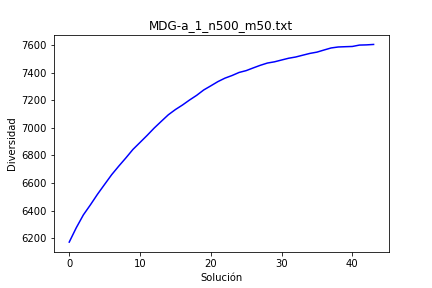
\includegraphics[width=57.5mm]{imgs/LS2Evol/LS2EMDG-a-1-n500-m50}}
	\subfigure{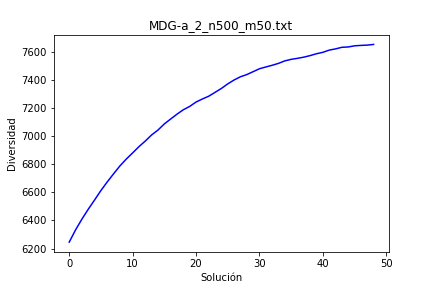
\includegraphics[width=57.5mm]{imgs/LS2Evol/LS2EMDG-a-2-n500-m50}}
	\subfigure{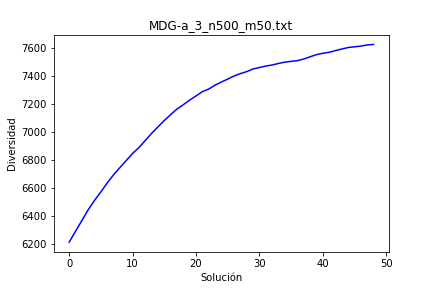
\includegraphics[width=57.5mm]{imgs/LS2Evol/LS2EMDG-a-3-n500-m50}}
	\subfigure{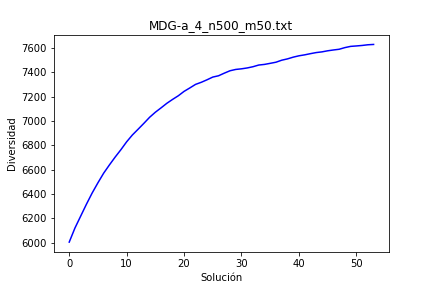
\includegraphics[width=57.5mm]{imgs/LS2Evol/LS2EMDG-a-4-n500-m50}}
	\subfigure{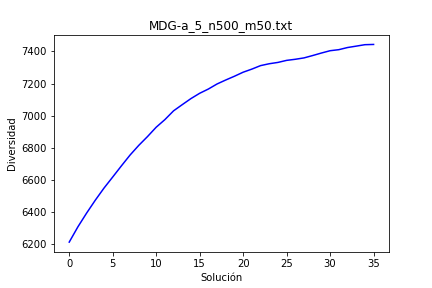
\includegraphics[width=57.5mm]{imgs/LS2Evol/LS2EMDG-a-5-n500-m50}}
	\subfigure{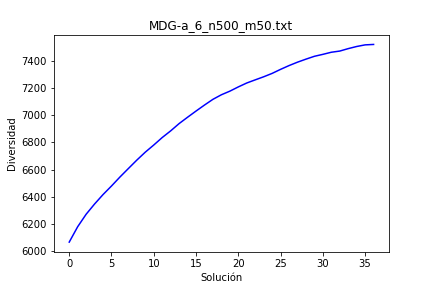
\includegraphics[width=57.5mm]{imgs/LS2Evol/LS2EMDG-a-6-n500-m50}}
	\subfigure{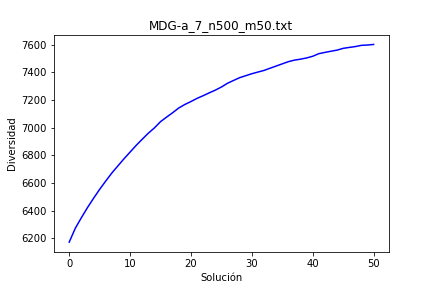
\includegraphics[width=57.5mm]{imgs/LS2Evol/LS2EMDG-a-7-n500-m50}}
	\subfigure{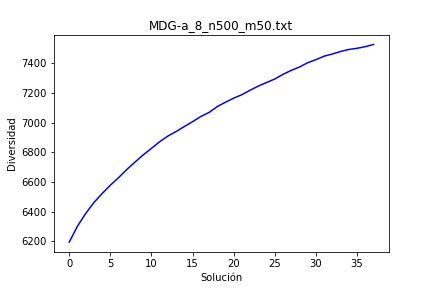
\includegraphics[width=57.5mm]{imgs/LS2Evol/LS2EMDG-a-8-n500-m50}}
	\subfigure{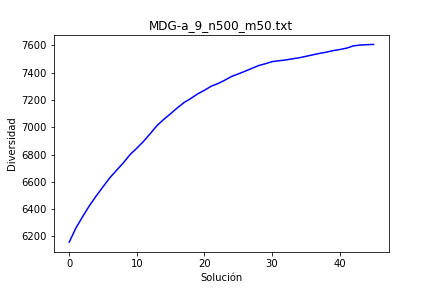
\includegraphics[width=57.5mm]{imgs/LS2Evol/LS2EMDG-a-9-n500-m50}}
	\subfigure{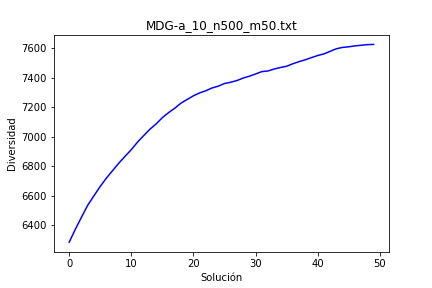
\includegraphics[width=57.5mm]{imgs/LS2Evol/LS2EMDG-a-10-n500-m50}}
	\caption{Gráficas de convergencia de BL con Mejor en los ejemplos del grupo MDG-a.}
	\label{fig:graph-bl-best-a}
\end{figure}

\begin{figure}[H]
	\centering
	\subfigure{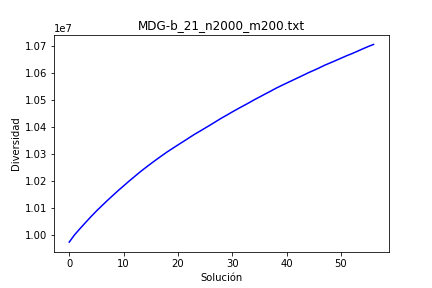
\includegraphics[width=57.5mm]{imgs/LS2Evol/LS2EMDG-b-21-n2000-m200}}
	\subfigure{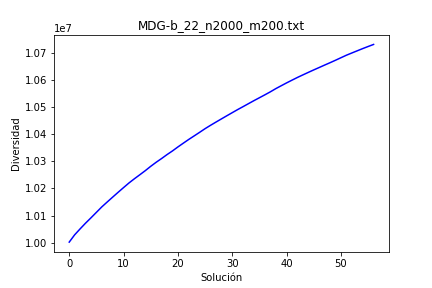
\includegraphics[width=57.5mm]{imgs/LS2Evol/LS2EMDG-b-22-n2000-m200}}
	\subfigure{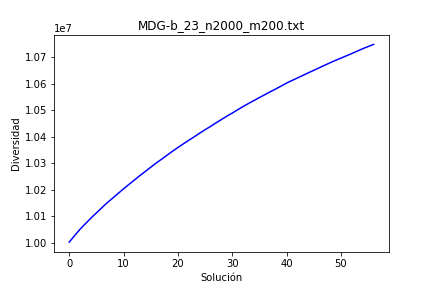
\includegraphics[width=57.5mm]{imgs/LS2Evol/LS2EMDG-b-23-n2000-m200}}
	\subfigure{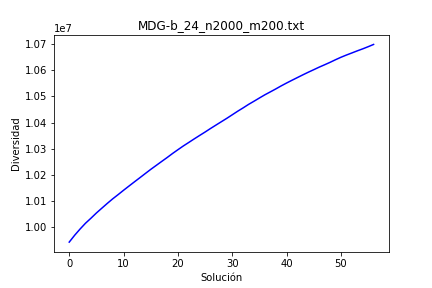
\includegraphics[width=57.5mm]{imgs/LS2Evol/LS2EMDG-b-24-n2000-m200}}
	\subfigure{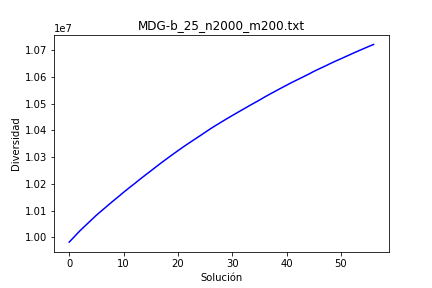
\includegraphics[width=57.5mm]{imgs/LS2Evol/LS2EMDG-b-25-n2000-m200}}
	\subfigure{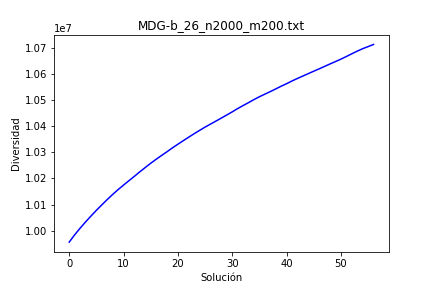
\includegraphics[width=57.5mm]{imgs/LS2Evol/LS2EMDG-b-26-n2000-m200}}
	\subfigure{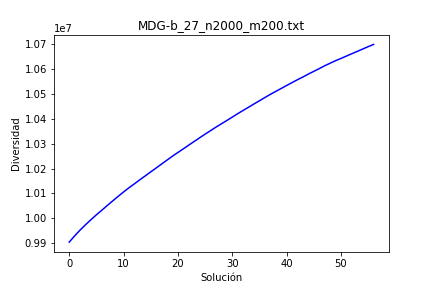
\includegraphics[width=57.5mm]{imgs/LS2Evol/LS2EMDG-b-27-n2000-m200}}
	\subfigure{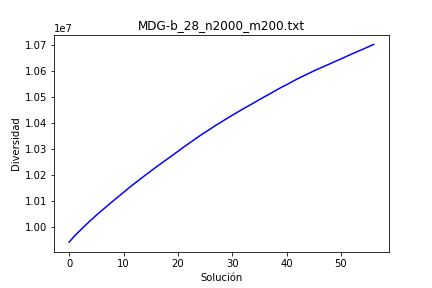
\includegraphics[width=57.5mm]{imgs/LS2Evol/LS2EMDG-b-28-n2000-m200}}
	\subfigure{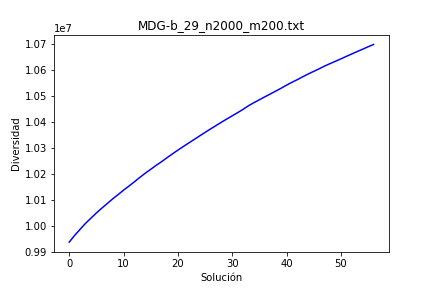
\includegraphics[width=57.5mm]{imgs/LS2Evol/LS2EMDG-b-29-n2000-m200}}
	\subfigure{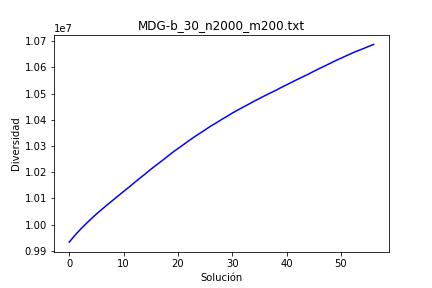
\includegraphics[width=57.5mm]{imgs/LS2Evol/LS2EMDG-b-30-n2000-m200}}
	\caption{Gráficas de convergencia de BL con Mejor en los ejemplos del grupo MDG-b.}
	\label{fig:graph-bl-best-b}
\end{figure}

\begin{figure}[H]
	\centering
	\subfigure{\includegraphics[width=57.5mm]{imgs/LS2Evol/LS2EMDG-c-1-n3000-m300}}
	\subfigure{\includegraphics[width=57.5mm]{imgs/LS2Evol/LS2EMDG-c-2-n3000-m300}}
	\subfigure{\includegraphics[width=57.5mm]{imgs/LS2Evol/LS2EMDG-c-8-n3000-m400}}
	\subfigure{\includegraphics[width=57.5mm]{imgs/LS2Evol/LS2EMDG-c-9-n3000-m400}}
	\subfigure{\includegraphics[width=57.5mm]{imgs/LS2Evol/LS2EMDG-c-10-n3000-m400}}
	\subfigure{\includegraphics[width=57.5mm]{imgs/LS2Evol/LS2EMDG-c-13-n3000-m500}}
	\subfigure{\includegraphics[width=57.5mm]{imgs/LS2Evol/LS2EMDG-c-14-n3000-m500}}
	\subfigure{\includegraphics[width=57.5mm]{imgs/LS2Evol/LS2EMDG-c-15-n3000-m500}}
	\subfigure{\includegraphics[width=57.5mm]{imgs/LS2Evol/LS2EMDG-c-19-n3000-m600}}
	\subfigure{\includegraphics[width=57.5mm]{imgs/LS2Evol/LS2EMDG-c-20-n3000-m600}}
	\caption{Gráficas de convergencia de BL con Mejor en los ejemplos del grupo MDG-c.}
	\label{fig:graph-bl-best-c}
\end{figure}

En los ejemplos del grupo MDG-a, la forma de las gráficas es similar a las que proporcionaba la estrategia del Primer Mejor, y 
la mejor también es similar. También es similar la mejora que consigue (eje de ordenadas) con respecto a la solución aleatoria.

En cambio, en los ejemplos de los grupos MDG-b y MDG-c, el crecimiento del valor de la función exponencial es prácticamente lineal,
sobre todo en los ejemplos más grandes. Además, en el eje de ordenadas observamos que la mejora que consigue este algoritmo en 
estos ejemplos respecto a la solución aleatoria es mucho menor, en los ejemplos grandes no llega al 2\% de la diversidad.

En el eje de abscisas, observamos que el número de actualizaciones del algoritmo BL con primer mejor es de entorno a 50,
independientemente del tamaño del problema. Esto podría significar que el algoritmo para antes de tiempo y no llega a explorar
el espacio de soluciones todo lo que podría, así que obtenemos una tabla con las llamadas a la función de evaluación de cada
estrategia.

La estrategia del Primer Mejor es capaz de parar en mitad de una iteración si se llega al límite de llamadas, mientras que la 
estrategia del Mejor la he diseñado para que se detenga al final de la iteración. Por este motivo, el algoritmo del Mejor puede
exceder el límite de llamadas, pero nunca en más de $n$, De modo que no tiene mucha importancia de cara a los tiempos de ejecución
y al comportamiento del algoritmo.

\begin{table}[H]
	\centering
	\begin{tabular}{|ccc|}
		\hline
		Caso & Primer Mejor & Mejor\\ \hline
		MDG-a\_10\_n500\_m50 & 4933 & 22500\\
		MDG-a\_1\_n500\_m50 & 3533 & 19800\\
		MDG-a\_2\_n500\_m50 & 2664 & 22050\\
		MDG-a\_3\_n500\_m50 & 1522 & 22050\\
		MDG-a\_4\_n500\_m50 & 1843 & 24300\\
		MDG-a\_5\_n500\_m50 & 1869 & 16200\\
		MDG-a\_6\_n500\_m50 & 2330 & 16650\\
		MDG-a\_7\_n500\_m50 & 2776 & 22950\\
		MDG-a\_8\_n500\_m50 & 3439 & 17100\\
		MDG-a\_9\_n500\_m50 & 2246 & 20700\\
		MDG-b\_21\_n2000\_m200 & 29153 & 100800\\
		MDG-b\_22\_n2000\_m200 & 23745 & 100800\\
		MDG-b\_23\_n2000\_m200 & 28631 & 100800\\
		MDG-b\_24\_n2000\_m200 & 30061 & 100800\\
		MDG-b\_25\_n2000\_m200 & 22374 & 100800\\
		MDG-b\_26\_n2000\_m200 & 40168 & 100800\\
		MDG-b\_27\_n2000\_m200 & 31362 & 100800\\
		MDG-b\_28\_n2000\_m200 & 15585 & 100800\\
		MDG-b\_29\_n2000\_m200 & 25351 & 100800\\
		MDG-b\_30\_n2000\_m200 & 19936 & 100800\\
		MDG-c\_10\_n3000\_m400 & 34032 & 101400\\
		MDG-c\_13\_n3000\_m500 & 27872 & 100000\\
		MDG-c\_14\_n3000\_m500 & 47459 & 100000\\
		MDG-c\_15\_n3000\_m500 & 79989 & 100000\\
		MDG-c\_19\_n3000\_m600 & 34607 & 100800\\
		MDG-c\_1\_n3000\_m300 & 58816 & 102600\\
		MDG-c\_20\_n3000\_m600 & 44010 & 100800\\
		MDG-c\_2\_n3000\_m300 & 63615 & 102600\\
		MDG-c\_8\_n3000\_m400 & 60814 & 101400\\
		MDG-c\_9\_n3000\_m400 & 51098 & 101400\\
		\hline
	\end{tabular}
	\caption{Número de llamadas a la función de evaluación por las estrategias Mejor y Primer Mejor para cada ejemplo.}
	\label{tab:calls}
\end{table}

Efectivamente, comprobamos que la estrategia del Primer Mejor siempre alcanza un máximo local. En cambio, la del Mejor
invierte demasiadas evaluaciones en cada iteración de los ejemplos grandes, lo que provoca que pare antes de alcanzar uno.

Por el contrario, el número de barajamientos de los candidatos que realiza la estrategia del Mejor es mucho menor, ya que
actualiza la solución menos veces. Este algoritmo invierte prácticamente todo su tiempo de ejecución en llamadas a la función
de evaluación.

Tras observar esto, es probable que al quizar o aumentar el límite de llamadas a la función de evaluación, el la estrategia del 
Mejor se asemeje en eficacia a la del Primer Mejor. No obstante, en los ejemplos del grupo MDG-a, donde ambos algoritmos se
 ejecutan al completo, la desviación que logra
la estrategia del Primer Mejor es ligeramente menor. Además, la mejor que realiza el algoritmo Primer Mejor respecto al tiempo que
tarda sugiere que la estrategia Mejor necesitaría más tiempo para alcanzar soluciones de la misma calidad.

Finalmente, hay que tener en cuenta que en otros problemas donde no sea posible la factorización de la función de evaluación,
la estrategia del Mejor sería mucho más lenta que la del Primer Mejor. Debido a que la mayoría de su tiempo se dedida a evaluar
esta función.

Por tanto, concluimos que la estrategia del Mejor no parece ser tan mala como muestra la Tabla \ref{tab:comparativa-bs}, pero
es más conveniente actualizar más a menudo la solución en lugar de realizar exhaustivas búsquedas por el entorno de cada solución,
sobre todo si no se pudiese factorizar la función de evaluación.

\end{document}
